\section{System Design}
This chapter will describe SANSURGIMS, ``SAN Surgical Information Management System", which embodies the results of the project. The overarching goal of the project was to design a computer based handover prototype for clinical staff as outlined in \ref{Project Objectives}. The prototype that was produced in the course of this project is the first attempt within the hospital to create a computerised handover and as such required the student to analyse the current processes as well as undertake a requirements analysis of the handover process. The requirements analysis was accompanied by the gathering of all paper based forms used on the ward. Together, these three aspects represented the design drivers for the project. Each of these aspects is described in more detail in the following pages.   

\subsection{Handover Overview}
Before undertaking any kind of design work, it was necessary for the student to understand and analyse the current handover processes employed on the ward.   The handover between nurses, in the formal sense, takes place three times a day, once for each shift. Handover is held at 7 am, 2 pm and 10 pm. The handover takes place in the staff lounge room on the ward. The purpose of the handover is to transfer information about the patients on the ward from one shift to the next. This is especially important in patient care because the handover process enables nurses to highlight important information about a patient that a nurse that is starting her shift \textbf{must} know in order to properly care for her assigned patients as well as to properly plan her shift. The information sources for any type of handover, not just the nurse to nurse handover, are diverse as are the communication channels employed as depicted by the figure below.
\newpage
\begin{figure}[hp]
				\centering
				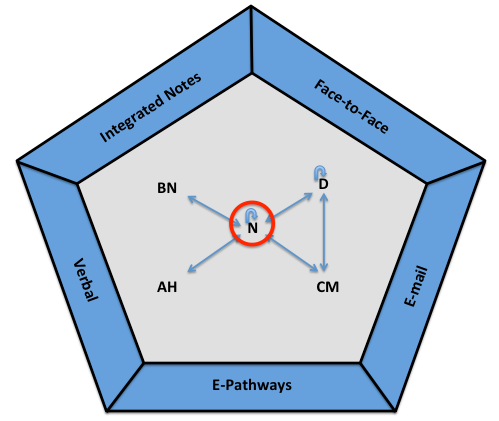
\includegraphics[scale=1.0, width=90mm]{Images/Clinical_Handover_Overview}
				\caption{Clinical Handover Overview}
\end{figure} 

\noindent As the figure shows, there are five information sources that are also utilised as communication channels. Face-to-Face and verbal communication is the quickest and most efficient way of relaying information in a clinical setting. This is emphasised by the fact that clinical staff have very little time during their shift that isn't devoted to patient care. Thus, communication usually occurs ad-hoc and spur of the moment whenever staff have a minute to spare. This includes communication with doctors, other wards and other nurses. Another advantage of using face-to-face and verbal communication is the fact that clinical staff can obtain immediate feedback to their questions or information exchange. This allows staff to quickly act on information instead of wasting time waiting. This is also one of the reason why handover is being done in a verbal, usually face-to-face, manner on the ward. 
\\ \\
As stated, handover should focus on highlighting vital patient information and thus, the nurses and other clinical staff still need to go back to documented information sources to obtain a complete picture of the patient. Such documented information includes a patient's integrated notes or e-pathways as is the case on the surgical ward. A patient's integrated notes is a folder containing all the information in regard to the patient such as filled out paper based forms, doctors orders, medication orders, etc. The integrated notes thus represent everything that is known about a patient. While most wards at the SAN still use paper based integrated notes, the surgical ward has moved to an electronic system called e-Pathways, which stores all patient information electronically. In essence, e-Pathways is the electronic equivalent of a patient's integrated notes. It should also be mentioned that these integrated notes are used by all clinical staff that are charged with the care of the patient including case managers and if relevant breast navigators. This leads to the natural conclusion that it is also used as a communication medium between staff albeit a slow one. This is especially the case for any non-nursing staff as they are not on the ward at all times and the nurse caring for a patient might not be around at the time so information is written into the notes that the nurse needs to read. This in turn leads to the necessity that the nurse go through the integrated notes or e-Pathways of her patients several times a day to check for new information, something that is rather tedious and time consuming and takes the nurse away from her primary duty of patient care.
\\ \\
The last communication channel and source of information is e-mail. This channel is not used in regard to handover information but was added for completeness sake. E-mail is usually used by doctors or breast navigators between each other. It also depends on personal preference whether or not e-mail is used. 
\\ \\
As can be seen by the variety of communication channels and information sources, it is quite a difficult task to transform the current processes into an electronic form. Needless to say this would require a change, depending on each staff member this could be a drastic change, in how handover is done and how information is handled within the hospital. This will be discussed further in XXX.

\subsection{Current Handover Process}
This section will outline and describe the current handover process for a nurse to nurse handover taking place during a shift change. There are two points of concern with the current handover process that needed to be addressed by the prototype. The first point of concern is the fact that currently, nurses will add ``fluff" information to their handover. This ``fluff" is any and all information that is not vital information about the patient. This fluff ranges from repeating information to mentioning things such as ``the patient is moody". This fluff is not only irrelevant information in regard to handover but it also consumes time during handover and forces the nurses of the oncoming shift to hear information that they must actively filter out.
\\ \\
The second aspect of concern is the fact that nurses on occasion only write down handover information for the patients they are responsible for. This means that the nurse is only aware of her own patients thus limiting her ability regarding other patients on the ward. A situation in which this limited knowledge of patients on the ward becomes an issue is for example when family members of patient come onto the ward and request information about the person they want to see. If a nurse does not take down handover information for that patient then she cannot be the family members the information they seek and instead has to say ``I don't know, let me get someone who does". This negatively represents the work of the nurses and that of the hospital. Another kind of situation in which the lack of patient knowledge causes problems is if emergency action must be taken for a patient. If the nurse that is responsible for the patient in distress is not available, another nurse must take her place and action the care necessary. This can only be done if the nurse is aware of the relevant patient information. While this situation is very rare it is nevertheless a possibility and should be handled appropriately. 
\\ \\
Before describing the current handover process, it is necessary to describe the two main roles that partake in the handover. The two roles are the Team Leader (TL) and the Nurses. The roles have the following responsibilities: \\ \\

\hfil\begin{tabular}{|p{7cm}|p{7cm}|}
\hline
{\hfil\bf Team Leader} & {\hfil\bf Nurse} \\
\hline
\vspace{-5mm}\begin{itemize}
\item looks after ward
\item checks to make sure registered nurses (RN) are fine
\item is also a nurse
\item calls out \gls{NFR} status to all other nurses during handover
\item in contact with the Assistant Director of Nursing (ADON)
\end{itemize} & 
\vspace{-5mm}\begin{itemize}
\item primary carer of patients
\item handover to next shift
\item administer medication
\item fill out patient forms such as Observation Chart and Nursing Care Record
\item the night shift creates roster
\end{itemize} \\ 
\hline
\end{tabular}

\newpage
\noindent When the TL comes on for duty, he or she will check each patient to see what their NFR status is. This is recorded in the patient's integrated notes, not on e-pathways. Before the start of each shift, the nurses of the on-coming shift meet in the staff room for handover. The handover usually last around 30 minutes. All of the nurses on the on-coming shift remain in the room during the entire handover. 
\\ \\ 
The first thing that happens is that the TL tells all the nurses which of the patients are NFR. Afterwards, the TL assigns each nurse a set of patients for that shift, which the nurses mark on their Patient Handover List (see Appendix \ref{Patient Handover List}). Then the nurses from the off-going shift come in, usually one by one, and verbally tell everyone in the room about the patients they were responsible for. Each nurse does her handover a little differently even though there are guidelines for handover. They tell everyone the room number, patient name, short history, diagnosis, test results, medication changes, treatment changes, drug allergies as well as outstanding test results and tests/procedures that will occur that day. They report on any variances in vital signs, bowels, or any complications that the patient has. They also mention how the patient is feeling, if they are annoyed, sleepy, disoriented and other general information such as non-critical allergies, ie. shell fish allergy. If a patient is being discharged, the nurse will say where that patient is going and if the patient has left the hospital already, he or she is stricken from the list by the on-coming nurses. 
\\ \\
The nurse who is responsible for that patient on the next shift writes down the important information on her Patient Handover List. The nurse will also create a small schedule of upcoming tests and procedures so that she can plan her shift accordingly and not be pressed for time during the shift. Any nurse can ask questions about the patient and the off-going nurse will try to answer them. If a patient is not assigned to a nurse, that nurse will not write down patient information. Should there be any doctor's notes or orders, then these are also mentioned during the handover process. When the off-going nurse is finished giving her handover she leaves the room and thus ends her shift. Should any information be missing then the on-coming nurse will check e-Pathways, the integrated notes or contact the relevant person in the hospital.
\\ \\
Below is a process diagram depicting how handover is currently undertaken based on the previous description.

\begin{figure}[hp]
				\centering
				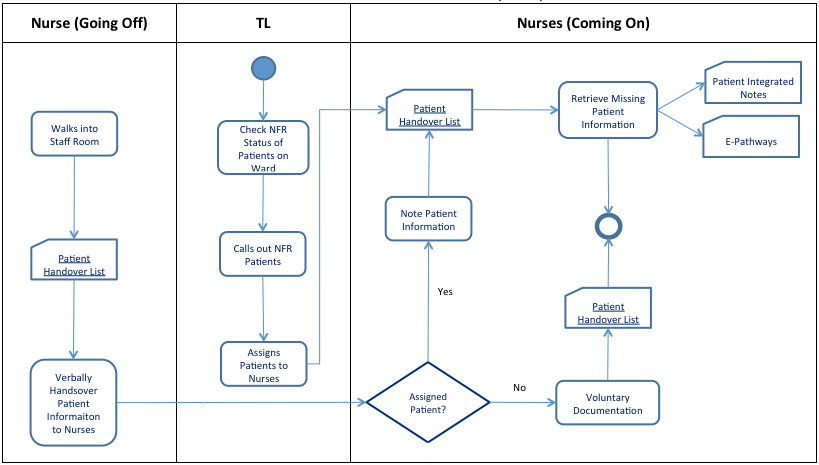
\includegraphics[angle=-90,scale=1.0, width=120mm]{Images/Nurse-to-Nurse-Handover-Process-As-Is}
				\caption{Current Nurse-to-Nurse Handover}
\end{figure} 
\newpage

\subsection{Requirements Analysis}
Concurrently to understanding the current handover process, the student undertook a requirements analysis for handover. The student interviewed various clinical staff fulfilling varying roles within the hospital. For a complete list of roles encountered during the requirements analysis see Appendix \ref{User Roles}. The interviews allowed the student to better understand the various roles within the hospital as well as obtaining the view on handover from the major roles involved in handover. After having undertaken the interviews, the student compiled a requirements document that was then verified by staff. 
\\ \\ 
The student based his requirements model on that of the Business Analyst Body of Knowledge (\cite{IIBA}). The requirements were split into business, stakeholder, pre-requisite requirements, functional and non-functional requirements. Pre-requisite requirements were requirements that must be fulfilled in order to design a clinical handover and refer to various paper based forms obtained throughout the project.  The requirements are documented in Appendix \ref{Handover Requirements}.
\\ \\
It should be noted that the requirements gathered and documented are an attempt to fully document handover requirements and thus are not limited to requirements that can be fulfilled by iCIMS. An example where this is the case is with printing the handover information. While iCIMS has a print function, it merely prints out the web page content and does not allow for print styling. Printing out the web page handover would not aid the nursing staff in their work as each patient would reside on a separate printed page. Nurses would have to carry around seven to fifteen pages worth of patient information, which is not something that is feasible. Instead, the information system containing the handover should be able to print a handover list such as the one currently employed by the nurses.

\subsection{Form Gathering}
As part of the requirements analysis the student collected all forms in use on the ward. All forms were collected in order to identify the sources of information that ultimately is handed over between shifts. The student collected over twenty forms during the requirements analysis. After collecting all of the forms, the student went through all the forms and identified the ten most important forms in regard to handover. This was done in order to keep within the scope of the project and to reduce the number of forms to a number that could be managed by the students in regard to analysis and digitisation. Of all the forms collected, the following ten forms were deemed most important by the student in conjunction with clinical staff, in no specific order:

\begin{enumerate}
\item Nursing Care Record Form
\item Fluid Balance Chart Form
\item Intravenous Fluid Orders Form
\item Pain \& Symptom Assessment Form
\item Patient History Form
\item Adult Observation Chart
\item Medication Chart Form
\item Temporary Transfer/Handover Form
\item Patient Handover List Form
\item Patient Mobility Form
\end{enumerate}

\noindent Apart from forms 5 and 8, all forms are filled out at least once a day and thus hold the most up to date information on the patient. In order to better understand the forms and how the relevant information is documented, the student also gathered filled-in versions of these forms. A very important issue to raise here is the fact that because the forms are paper based, they are filled out by hand leading to issues with legibility. The student, on numerous occasions, encountered this problem and had to seek assistance from the relevant staff member to clarify noted information. The issue of legibility was also raised by clinical staff themselves, not only in regard to doctors but to all staff, and is something that they wished to be addressed. The filled-in forms also allowed the student to enter realistic data into the prototype in order to present the functionality to clinical staff.
\\ \\
Another issue that should be noted in regard to forms is the fact that most of the time, certain parts of forms were not filled out because they were not relevant for that patient. This presented the student with the problem that diverse variations of information was not available for all parts of forms. Unfortunately, it was unrealistic to ask clinical staff to provide such information for all possible situations because that would have required them to use a considerable amount of their time to generate the information, time that they did not have. Nevertheless, the student managed to adequately design the prototype based on the available information.

\subsection{Design Process}
As described in \ref{Overview}, the student utilised an incremental and iterative user driven development model. The realisation of the development model with iCIMS is depicted below.

\begin{figure}[hp]
				\centering
				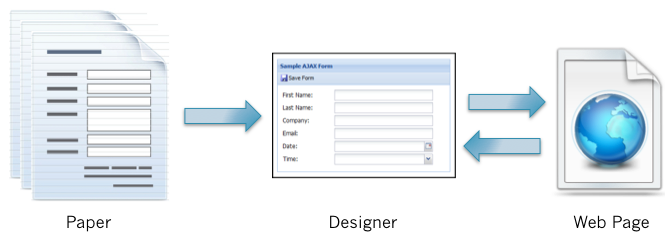
\includegraphics[scale=1.0, width=120mm]{Images/Design-Process}
				\caption{Design Process}
\end{figure} 

\noindent The first step undertaken was to digitise the paper forms within iCIMS. This meant attempting to copy the form's design and layout one to one. The reason why the forms were copied one to one was so that the student did not influence the design of the system and that the clinical staff could partake in all design steps. The one to one copy of the form also allowed the clinical staff to more easily identify the form being displayed in the system. It also allowed the student to more easily elicit staff feedback because the staff were not confused by looking at something totally new. After seeing the digital copy of the form, the clinical staff could then identify shortcomings of the forms themselves and, together with the student, undertake changes to the forms. The digitised forms were displayed in the web browser and it was based on the web page display that the clinical staff gave feedback and suggestions. 
\\ \\
This process allowed the student to incrementally add new forms into the designer and iteratively shape and mould these forms as desired with the help of the clinical staff. 

Describe figure of how you designed: paper-designer-web page
Give an example (Nursing Care Record) -> NEED TO SCAN THIS!
SCAN EMPTY HANDOVER LIST AS WELL

Describe design choices
Describe how you have to weight off between "Handover by Exception" and providing all relevant information to medical students/temp nurses/junior nurses that don't necessarily know what is normal

\subsection{User Scenarios}
Describe NEW process and its shortcomings (include Diagram)
how do users interact with the system? What operations do they perform?

